\subsection{Dataset creation}
We applied the methodology described earlier to hockey broadcast images. We generated our dataset, which contains images (inputs) and masks (outputs), by ourselves. To do so, we annotated a total of 43 NHL broadcast images. For the annotation part, we used an open source tool called \href{https://github.com/opencv/cvat}{cvat tool}. That tool allowed us to draw polygons around our labels and then associate a class to each pixels in the image.

To choose our labels, we used an iterative approach where we first used our judgment to decide arbitrary categories (ex: ice, crowd, corners, horizontal lines, vertical lines). After that, we used one single image and tried to fit a model using those labels. We then noticed the bahviour of the model regarding those categories and adapted them. For example, we noticed the corners, the horizontal and vertical lines such as the board were difficult to distinguish for the model. As such, we decided to merge them and use one single category called "board". Here are the \textbf{9 categories} we selected at the end: ice, boards, crowd, red line, blue lines, goal lines, circles in end zone, circles in neutral zone and dots. The figure \ref{fig:labeling} is an example of image we extracted and then labeled using our 9 categories.

\begin{figure}[H]
	\centering
	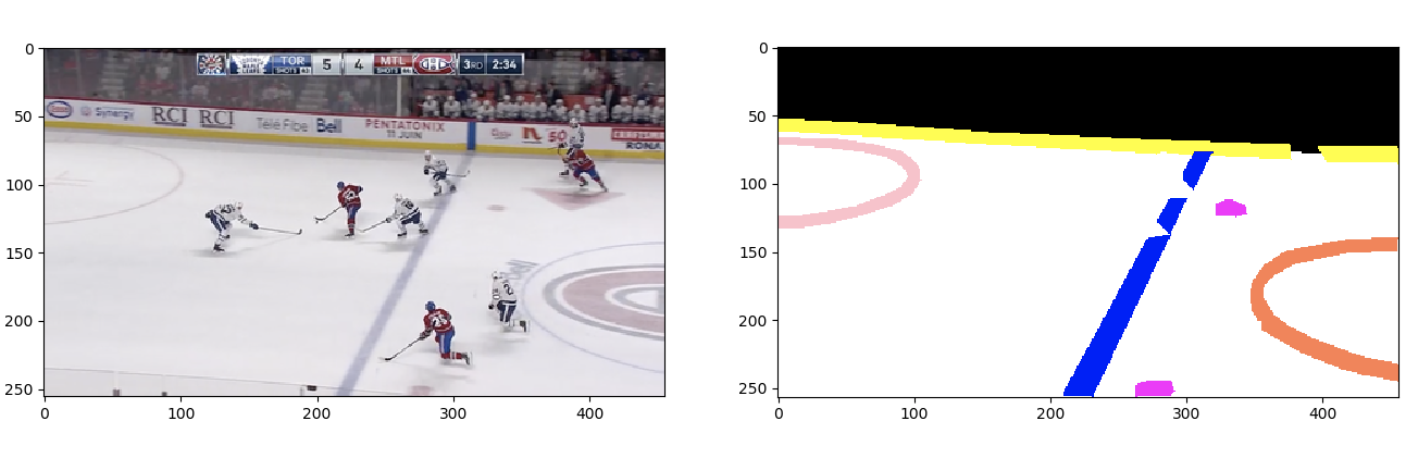
\includegraphics[width=8cm, height=4cm]{figures/labeling-example.png}
	\caption{Example of extracted image (left) and the labeling output (right) using the 9 categories.}
	\label{fig:labeling}
\end{figure}

In the methodology section, we mentionned we had a class imbalance problem. In that section, we tackled this problem by adapting the loss. In the labeling task, we also tackled that class imbalance problem by subjectively drawing larger polygons for rare categories such as dots or circles.
